% !TeX TS-program = Lualatex
% !TeX encoding = UTF-8 Unicode
% !TeX spellcheck = en
% !BIB TS-program = bibtex
% -*- coding: UTF-8; -*-
% vim: set fenc=utf-8
%%%%%%%%%%%%%%%%%%%%%%%%%%%%%%%%%%%%%%%%%%%%%%%%%%%%%%%%%%%%%%%%%%%%%
% 
\documentclass[runningheads]{llncs}
%
\usepackage[T1]{fontenc}
%
% \usepackage[utf8]{inputenc}
% \usepackage{times}
% \usepackage{wrapfig}
\usepackage{graphicx}
% \usepackage{floatrow}
% \usepackage{multicol}
\usepackage{amssymb}
\usepackage{amsmath}
\usepackage{hyperref}
\usepackage{siunitx}
%%%%%%%%%%%%%%%%%%%%%%%%%%%%%%%%%%%%%%%%%%%%%%%%%%%%%%%%%%%%%%%%%%%%%
% NOTATIONS
% Pixel world
\newcommand{\presynaddr}{a} % pre address
\newcommand{\postsynaddr}{b} % post address
\newcommand{\numevent}{N_{ev}} % total number of events
\newcommand{\presynaddrspace}{\mathcal{A}} %presynaptic address space
\newcommand{\postsynaddrspace}{\mathcal{B}} %postsynaptic address space
\newcommand{\Npol}{N_\text{p}} % number of polarity
\newcommand{\Nneuron}{N_\text{n}} % number of output neurons in the layer
\newcommand{\arank}{r} % address index
\newcommand{\bias}{b} % bias for the MLR model
\newcommand{\synapse}{\mathcal{S}} % synapse
\newcommand{\synapticweight}{w} % synaptic weight
\newcommand{\synapticdelay}{\delta} % synaptic delay
\newcommand{\ranksyn}{s} % synapse index
\newcommand{\Nsyn}{N_{s}} % total number of synapses
\newcommand{\activeweights}{\mathcal{W}} 
\newcommand{\timev}{t} % time
\newcommand{\polev}{p} % polarity
\newcommand{\event}{\epsilon} % event
\newcommand{\eventstream}{\xi} % stream of events
\newcommand{\TS}{S} % time surface
\newcommand{\neuron}{\mathbf{n}} % neuron in the SNN (defined by the spatial position and the channel)
\newcommand{\postneuron}{\mathbf{m}} % post synaptic neuron in the SNN (defined by the spatial position and the kernel)
\newcommand{\channel}{\mathbf{p}} % channel
\newcommand{\layer}{\mathbf{L}} % layer
\newcommand{\ms}{\si{\milli\second}}%
\newcommand{\us}{\si{\micro\second}}%
\newcommand{\timecontext}{T} % time context (cf HOTS) matrice gathering last event times
\newcommand{\current}{I} % post synaptic current
\newcommand{\volt}{u} % membrane potential
\newcommand{\volts}{V} % matrix of membrane potentials
\newcommand{\gain}{\gamma} % homeostatic gain
\newcommand{\simil}{\beta} % similarity value
\newcommand{\Nclass}{N_\text{class}} % number of classes for MLR:
\newcommand{\Nx}{N_\text{X}}
\newcommand{\Ny}{N_\text{Y}}
\newcommand{\Ntime}{N_\text{t}}
\newcommand{\kernel}{K} % convolution kernel
%\newcommand{\kernelind}{\mathbf{k}} % indice of the kernel
\newcommand{\kernelind}{k} % indice of the kernel
\newcommand{\Kx}{K_\text{x}}
\newcommand{\Ky}{K_\text{y}}
\newcommand{\Ktime}{K_\text{t}}
\newcommand{\classiflayer}{\mathbf{C}}
\newcommand{\class}{c} % class k of the MLR
\newcommand{\lrweights}{\theta} % matrix of MLR weights
\newcommand{\lrtrue}{y} % true value of the prediction for MLR
\newcommand{\loss}{J} % cost function for MLR
\newcommand{\softmax}{\sigma}
\newcommand{\actfreq}{f}
\newcommand{\decision}{\hat{y}}
\newcommand{\colorsec}{black}
\newcommand{\colorsubsec}{black}
\newcommand{\speed}{v}
\newcommand{\Nspeed}{N_v}
% Example definitions.
% --------------------
\def\x{{\mathbf x}}
\def\L{{\cal L}}
\newcommand{\fig}[1]{Fig.~\ref{fig:#1}}%{Figure~\ref{fig:#1}}
\DeclareMathOperator*{\argmax}{arg\,max}
\DeclareMathOperator*{\argmin}{arg\,min}

%%%%%%%%%%%%%%%%%%%%%%%%%%%%%%%%%%%%%%%%%%%%%%%%%%%%%%%%%%%%%%%%%%%%%%
% \usepackage{natbib}
% \usepackage[
% %style=chem-acs,
% style=numeric,						% numeric style for reference list
% citestyle=numeric-comp,
% %style=alphabetic-verb,
% giveninits=false,
% maxbibnames=1,
% %firstinits=true,
% %style=apa,
% %maxcitenames=1,
% %maxnames=3,
% %minnames=1,
% %maxbibnames=99,
% dateabbrev=true,
% giveninits=true,
% %uniquename=init,
% url=false,
% doi=false,
% isbn=false,
% eprint=false,
% texencoding=utf8,
% bibencoding=utf8,
% autocite=superscript,boutin_effect_2020
% backend=biber,
% %sorting=none,
% sorting=none,
% sortcites=false,
% %articletitle=false
% ]{biblatex}%

% \bibliography{ref.bib}
%%%%%%%%%%%%%%%%%%%%%%%%%%%%%%%%%%%%%%%%%%%%%%%%%%%%%%%%%%%%%%%%%%%%%%
% \newcommand{\mycaption}[1]{\caption*{#1}}

% \usepackage{titlesec}
% % \titlespacing*{<command>}{<left>}{<before-sep>}{<after-sep>}
% \titlespacing*{\section}
% {0pt}{1.5ex}{0.8ex}
% \titlespacing*{\subsection}
% {0pt}{0.9ex}{0.4ex}
% \titlespacing*{\subsubsection}
% {0pt}{0.5ex}{0.3ex}
% \titlespacing*{\paragraph}{%
%   0pt}{%              left margin
%   0.0\baselineskip}{% space before (vertical)
%   1em}%               space after (horizontal)

% \usepackage{setspace}

\begin{document}

%%%-----------------------------------------------------------------
\title{Accurate detection of spiking motifs in multi-unit raster plots}

\author{Laurent U Perrinet\orcidID{0000-0002-9536-010X}\thanks{Funded by A*MIDEX grant AMX-21-RID-025 ``\href{https://laurentperrinet.github.io/grant/polychronies/}{Polychronies}''.}}
%
\authorrunning{LU Perrinet}
% First names are abbreviated in the running head.
% If there are more than two authors, 'et al.' is used.
%
\institute{INT UMR7289, Aix Marseille Univ, CNRS; 27 Bd Moulin, 13005 Marseille, France
% \url{https://laurentperrinet.github.io} \email{laurent.perrinet@univ-amu.fr}
}
%
\maketitle              % typeset the header of the contribution
%
\begin{abstract} Recently, there has been growing interest in the hypothesis that information can be carried within neural activity by precise spiking motifs. As a result, there have been several recent proposals for algorithms to detect such motifs in the Spiking Unit Activity (SUA) of populations of neurons. In this study, we introduce a detection model as an inversion of a generative model of raster plot synthesis. From this model, an optimal detection procedure is derived. This takes the form of a logistic regression coupled with a temporal convolution. Since this model is differentiable, we derive a supervised learning method in the form of gradient descent on the loss function of an auto-encoder model. We evaluate the ability of this model to detect spiking motifs in synthetic data. This learning method is able to recover the synthetically generated spiking motifs, and we plan to extend this method to neurobiological data as well.
%
\keywords{Neurobiology \and  spike trains \and population coding  \and spiking motifs \and heterogeneous delays \and pattern detection.}
\end{abstract}

%----------------------------%
\section{Introduction}
%---------------------------

%%%%%%%%%%%%%%%%%%%%%%%%%%%%%%%%%%%%%%%%%%%%%
\subsection{The age of large-scale neurobiological event-based data}
%%%%%%%%%%%%%%%%%%%%%%%%%%%%%%%%%%%%%%%%%%%%%
% 
Over the past decade, tremendous technological advances across multiple disciplines have dramatically expanded the frontiers of experimentally accessible neuroscience. % Bridging different spatial and temporal scales, combining \textit{in vivo} two-photon imaging, large population recording array technologies, optogenetic circuit control tools, transgenic manipulations, as well as large volume circuit reconstructions, 
These tools are now being used to probe the function, structure, and dynamics of neural networks at unprecedented levels of detail and precision. The staggering complexity of biological reality revealed by these technologies highlights the importance of neurobiological knowledge to provide a conceptual bridge between abstract principles of brain function and their biological implementation in neural circuits. As a consequence, there is a growing need to scale such analysis methods to larger amounts of data. 

There are several approaches that try to solve this problem. One algorithm capable of accomplishing such a daunting task is the Rastermap algorithm~\cite{pachitariu_robustness_2018}. Basically, it rearranges neurons in the raster map based on the similarity of their activity and applies a deconvolution strategy based on a linear model. However, this method has mainly been tested on calcium imaging data, which is known to add some imprecision to the timing of the original spiking activity. 
% In~\cite{russo_cell_2017}, the authors developed novel machine learning tools and statistical tests for unsupervised spatiotemporal pattern detection in non-stationary environments, which were applied to simultaneous electrophysiological recordings from tens to hundreds of neurons to decode cognitive processes from neural activity. Overall, this provides evidence for the importance of such machine-learning based tools to provide breakthroughs in neuroscience.

% In the paper by~\cite{russo_cell_2017}, the authors present a unifying methodological and conceptual framework that detects assembly structure at many different timescales, levels of precision, and with arbitrary internal organization. 
To overcome the limitations of models that either require spike times to be discretized, use a suboptimal least-squares criterion, or do not provide uncertainty estimates for model predictions or estimated parameters, Williams {\it et al}~\cite{williams_point_2020} addresses each of these shortcomings by developing a point process model that characterizes fine-scale sequences at the level of individual spikes and represents sequence occurrences as a few marked events in continuous time. %As originally introduced by~\cite{kass_statistical_2005}, they use learnable time-warping parameters to model sequences of different durations that have been experimentally observed in neural circuits, and demonstrate these advantages on experimental recordings from the songbird higher vocal center and the rodent hippocampus. 
%
%%%%%%%%%%%%%%%%%%%%%%%%%%%%%%%%%%%%%%%%%%%%%
\subsection{Decoding neural activity using spike distances}
%%%%%%%%%%%%%%%%%%%%%%%%%%%%%%%%%%%%%%%%%%%%%
%
Overall, these methods rely on the definition of metrics to compute the distance between spike trains.
% There are several solutions to provide a distance between two given spike trains. 
One well-known measure is the Victor-Purpura distance, which overcomes inconsistencies experienced with a firing rate (Poisson model) of spike trains~\cite{victor_nature_1996}.
% 
A further study attempts to refine the metric by including a time constant as a parameter which is then used to interpolate the distance between a coincidence detector and a rate difference counter~\cite{van_rossum_novel_2001}. Such distances have been extended to non-Euclidean metrics and to the use of morphological manipulations to compute spike train dissimilarity~\cite{kreuz_measuring_2007}. These observations lead to the intuition that any distance may be the optimal solution of a generative model for these measures, possibly through non-linear relations~\cite{aronov_non-euclidean_2004}. 

Regarding spike timings, Levakova {\it et al}~\cite{levakova_review_2015} have reviewed existing methods for estimating the latency of neural responses that include Bayesian binning. Alternatively, unitary event analysis can be performed using a statistical model of chance detection~\cite{grun_unitary_2002-1}. This has been used extensively to detect significant synchronous patterns above chance~\cite{grun_unitary_2010}, especially in recordings of neuron pairs (see~\cite{riehle_spike_1997} for example). %This has recently been extended in~\cite{stella_3d-spade_2019} to find reoccurring patterns in parallel spike train data and determine their statistical significance. 
Including the possible existence to a temporal dithering of spike times improves the performance in the presence of patterns with different durations, such as surrogates generated to evaluate precisely timed higher order spike correlations~\cite{stella_comparing_2022}. % include sotomayor-vinck spike Ship
%
%%%%%%%%%%%%%%%%%%%%%%%%%%%%%%%%%%%%%%%%%%%%%
\subsection{Detecting spiking motifs with a heterogeneous delays SNN}
%%%%%%%%%%%%%%%%%%%%%%%%%%%%%%%%%%%%%%%%%%%%%
%
% We believe that the detection of spiking motifs should be based on a proper understanding of spiking neural networks (SNNs). However, most existing SNNs, especially those adapted from analogous deep learning like architectures, rely on encoding information based on a continuously varying firing rate.
% Notable exceptions of SNNs using precise spike timing are the time coding machine of~\cite{lazar_time_2004} and the 
These methods highlight the role of spike timing, and here, we propose a new metric inspired by the \textit{polychronization} model of Izhikevich~\cite{izhikevich_polychronization_2006}. This theoretical model is based on a random recurrent model of spiking neurons that includes synaptic delays chosen from a range of biologically realistic delays (from $0$ to $20~\ms$) and whose weights are evolving with a Spike-Time Dependent Plasticity (STDP) learning rule. Delays are defined as the total time taken for a spike to travel from the soma of one presynaptic neuron to that of the efferent postsynaptic neuron. Note that only the weights are changed using the STDP rule, and that the set of delays is randomly set at initialization and then ``frozen'' for the rest of the simulation. 

Due to the interplay between the delays and the STDP, the spiking neurons spontaneously self-organize into groups and %generate patterns of stereotypical polychronous activity, i.e., 
exhibit reproducible time-locked firing patterns, which the author defines as ``polychronous groups''. A key component of this model is the fact that the neurons in a group fire at different times, but because of the existence of heterogeneous delays, the spikes may converge at the postsynaptic neuron at the same time. This synchrony of arrival at the soma of the neuron leads to the summation of the excitatory postsynaptic potentials evoked by each spike, and thus to the crossing of the voltage threshold and the discharge of a spike (see Figure~\ref{fig:izhikevich}). According to the STDP rule, the group of neurons involved in this polychronous activity will see their synaptic weight increase and thus may consolidate the formation of a polychronous group.  A limitation of this model is that these heterogeneous delays are fixed and can not evolve in time.

%----------------------------%
%
\begin{figure}[t]
  \centering
  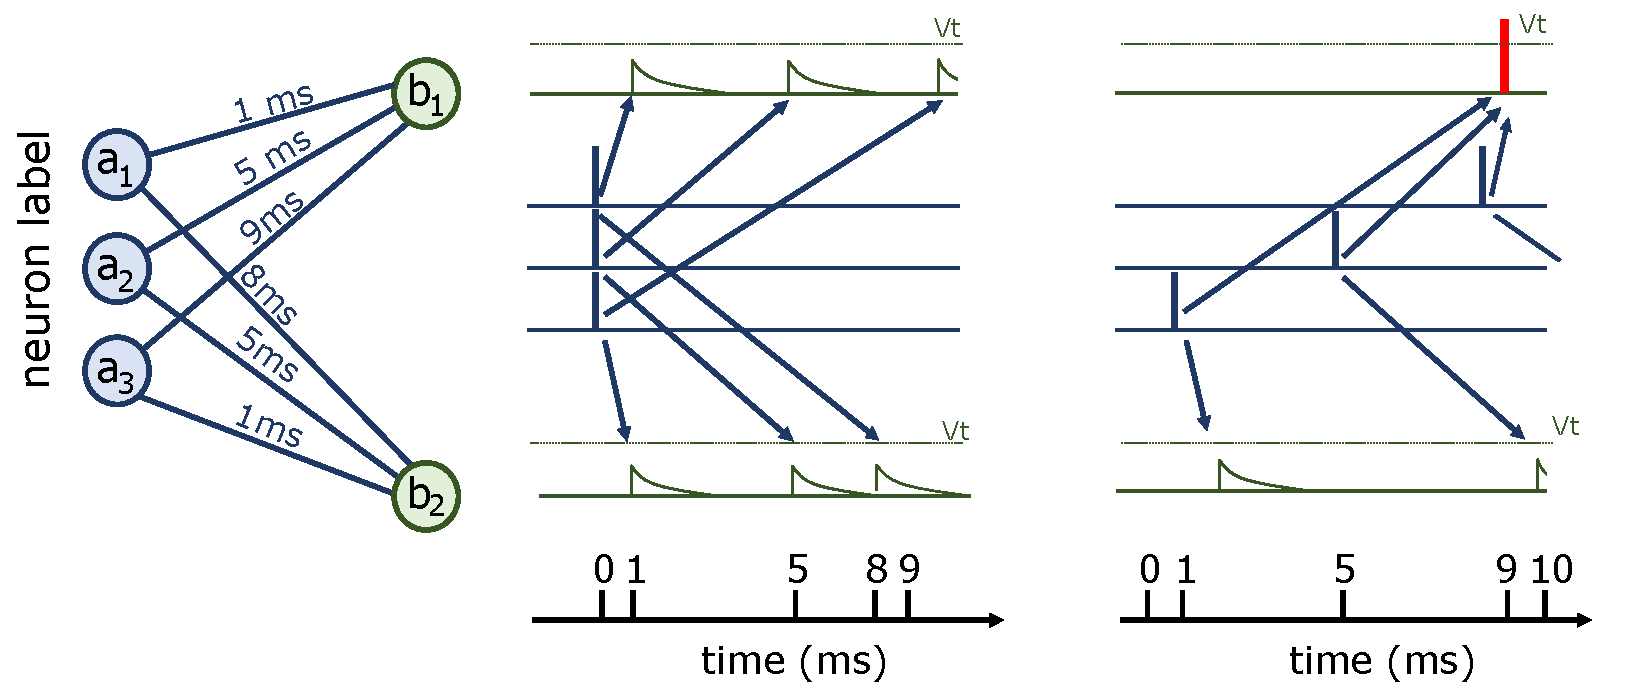
\includegraphics[width=0.95\linewidth]{figures/izhikevich.pdf}% https://www.overleaf.com/5625872443qpcwrkssgbsf
    \caption{\textbf{Core Mechanism of Spike Motif Detection.} \textit{(Left)}~In this toy example, three presynaptic neurons denoted \textit{a}$_1$, \textit{a}$_2$, and, \textit{a}$_3$ are fully connected to two postsynaptic neurons \textit{b}$_1$ and \textit{b}$_2$, with different delays of $1$, $5$, and $9~\ms$ for \textit{b}$_1$ and $8$, $5$, and $1~\ms$ for \textit{b}$_2$, respectively. \textit{(Middle)}~If three synchronous pulses are emitted from presynaptic neurons, this will generate postsynaptic potentials that reach \textit{b}$_1$ and \textit{b}$_2$ asynchronously because of the heterogeneous delays, and they may not be sufficient to reach the membrane threshold (dashed line) in either of the postsynaptic neurons. This is not enough to reach the membrane threshold of the post-synaptic neuron.  \textit{(Right)}~If the pulses are emitted from the presynaptic neurons in such a way that, taking into account the delays, they reach the post-synaptic neuron \textit{b}$_1$ at the same time (here, at $t=10~\ms$), the post-synaptic potentials $V_t$ evoked by the three presynaptic neurons sum up, causing the voltage threshold to be crossed and thus the emission of an output spike which signals the detection of a spiking motif in the presynaptic population (red color), while none is emitted by the post-synaptic neuron \textit{b}$_2$.
     }
  \label{fig:izhikevich}
\end{figure}
%----------------------------%

In this work, we propose to accurately detect spatio-temporal spiking motifs using a feed-forward, single layer heterogeneous delays spiking neural network  (HD-SNN). The paper is organized as follows. We develop a theoretically defined HD-SNN for which we can attune both the weights and delays. %We first detail the methodology by defining the basic mechanism of spiking neurons that utilize heterogeneous delays. 
This will allow us to formalize the spiking neuron used to learn the model's parameters in a supervised manner and test its effectiveness. In the results section, we will first evaluate the efficiency of the learning scheme. We will also study the robustness of the spiking motif detection mechanism and in particular its resilience to changing the dimensions of presynaptic, postsynaptic neurons, or the depth in the number of different possible delays. This will allow us to show how such a model can provide an efficient solution which may in the future be applied to neurobiological data.  %Finally, we will conclude by highlighting the main contributions of this paper, while defining some limitations which will open perspectives for future SNNs.  %In particular, as neuromorphic devices are by design good candidates for integrating computations over time, we highlight the fact that this event-driven algorithm is perfectly fit to be transferred to this type of hardware and to obtain significant gains in the energy which is used.
%
\section{Methods}
\label{sec:methods}
%%%-----------------------------------------------------------------
%%%-----------------------------------------------------------------
Let us formally define the Heterogeneous Delays Spiking Neural Network (HD-SNN). First, we will define raster plots in an event-based, then binarized setting. We will then derive a generative model for raster plots by way of a HD-SNN and deduce from this a model for the efficient detection of event-based motifs using a similar HD-SNN with ``inverted'' delays.
%
\subsection{Raster plots: from event-based to binarized}
%
In neurobiological recordings, %or in the sensory signal obtained from an event-based camera, 
any generic raster plot consists of a stream of \emph{spikes}. This can be formalized as a list of neural addresses and timestamps tuples $\event = \{(\presynaddr_\arank, \timev_\arank)\}_{\arank \in [1,\numevent]}$ where $\numevent \in \mathbb{N}$ is the total number of events in the data stream and the rank $\arank$ is the index of each event in the list of events. Each event has a time of occurrence $\timev_\arank$ which are typically ordered and an associated address $\presynaddr_\arank$ in the space $\presynaddrspace$ of possible addresses. In a neurobiological recording, this can be the identified set of neurons.

Events are generated by neurons which are defined on the one hand by the equations governing the evolution of its membrane potential dynamics on their soma and on the other hand by the integration of the synaptic potential propagatings on their dendritic tree. A classical characterization consists in detailing the synaptic weights of each synaptic contact, the so-called weight matrix. As we saw above, one may add heterogeneous delays, i.e., the precise timing from one afferent neuron's firing to its arrival in the soma. %, and how this changes the network's dynamics~\cite{izhikevich_polychronization_2006}. 
In such neurons, %we can parameterize each neuron by the set of tuples defining both the weight and the delay of each synaptic contact. As a consequence, a set of 
input presynaptic spikes $\event$ will be multiplexed in time by the dendrites defined by this synaptic set (see Figure~\ref{fig:izhikevich}). %, and notably by the respective delays which will multiplex in time all events. 

Let's formalize such a layer of spiking neurons with heterogeneous delays (HD-SNN). Each neuron $\postsynaddr \in \postsynaddrspace$  connects to presynaptic afferents from $\presynaddrspace$. In biology, a single cortical neuron has generally several thousands of synapses. Each may be defined by its synaptic weight and also its delay. %, that is, the time it takes for one spike to travel from the presynaptic neuron's soma to that of the postsynaptic neuron. %Neuron $\postsynaddr \in \postsynaddrspace$ is then described by the synaptic weights connecting it to a presynaptic afferent from $\presynaddrspace$ but also by the set of possible delays. 
Note that two neurons may contact with multiple synapses, and thus different delays. Scanning all neurons $\postsynaddr$, we thus define the set of $\Nsyn \in \mathbb{N}$ synapses  as  $\synapse = \{(\presynaddr_\ranksyn, \postsynaddr_\ranksyn, \synapticweight_\ranksyn, \synapticdelay_\ranksyn)\}_{\ranksyn \in [1,\Nsyn]}$, where each synapse is associated to a presynaptic address $\presynaddr_\ranksyn$, a postsynaptic address $\postsynaddr_\ranksyn$,  a weight $\synapticweight_\ranksyn$, and a delay $\synapticdelay_\ranksyn$. 

This defines the full connectivity of the HD-SNN model. Of particular interest is to define the receptive field of a postsynaptic neuron $\synapse^\postsynaddr =  \{(\presynaddr_\ranksyn, \postsynaddr_\ranksyn, \synapticweight_\ranksyn, \synapticdelay_\ranksyn) \| \postsynaddr_\ranksyn=\postsynaddr\}_{\ranksyn \in [1,\Nsyn]} $, or the emitting field of a presynaptic neuron $\synapse_\presynaddr =  \{(\presynaddr_\ranksyn, \postsynaddr_\ranksyn, \synapticweight_\ranksyn, \synapticdelay_\ranksyn) \| \presynaddr_\ranksyn=\presynaddr\}_{\ranksyn \in [1,\Nsyn]}$. Following this definition, an event stream which evokes neurons in the presynaptic address space is multiplexed by the synapses into a new event stream which is defined by the union of the sets generated by each emitting field from the presynaptic space: 
$ \cup_{\arank \in [1,\numevent]} \{ \{(\postsynaddr_\ranksyn, \synapticweight_\ranksyn, \timev_\arank + \synapticdelay_\ranksyn) \}_{ \ranksyn \in \synapse_{\presynaddr_\arank}} \}$. In biology, this new stream of events is naturally ordered in time as events reach the soma of post-synaptic neurons. In particular, when post-synaptic neurons are activated on their soma by this spatio-temporal motif, the discharge probability will increase, notably when these spikes converge on the soma in a synchronous manner. 

From the perspective of simulating such event-based computations on standard CPU- or GPU-based computers, it is useful to transform this event-based representation into a dense representation. Indeed, we may transform any event-based input as the boolean matrix $A \in \{0, 1 \}^{N\times T}$, where $N$ is the number of presynaptic neurons in $\presynaddrspace$ and $T$ is the number of time bins. In this simplified model, we will consider that heterogeneous delays are integers limited in range between $0$ and $D$ (that is, $\forall {\ranksyn \in [1,\Nsyn]}$, $0 \le \synapticdelay_\ranksyn \le D$) such that the synaptic set can be represented by the dense matrix $\kernel^\postsynaddr \in \mathbb{R}^{N\times D}$ giving for each neuron $\postsynaddr$ the weights as a function of presynaptic address and delay. It is equal to zero except on synapses: $\forall {\ranksyn \in \synapse^\postsynaddr}, \kernel^\postsynaddr(\presynaddr_\ranksyn,  \synapticdelay_\ranksyn) = \synapticweight_\ranksyn$. Equivalently, one may define for each presynaptic neuron $\presynaddr$ the emitting kernel as the transpose kernel $\kernel^T_\presynaddr \in \mathbb{R}^{M\times D}$, where $M$ is the number of postsynaptic neurons, whose values are zero except on synapses:  $\forall {\ranksyn \in \synapse_\presynaddr}, \kernel^T_\presynaddr(\postsynaddr_\ranksyn,  \synapticdelay_\ranksyn) = \synapticweight_\ranksyn$.

\subsection{A generative model for raster plots}

As described in Figure~\ref{fig:izhikevich}, a spiking motif can be detected using a properly tuned HD-SNN. Taking the argument the other way around, one may form a generative model for realistic raster plots in which any spikes in the presynaptic address space are generated by afferent spiking neurons and knowing that these are connected by a set of weights and delays whose structure is stable relatively to the coding timescale. When connection weights are strong and sparsely distributed, this firing will cause a specific temporal motif. Overall, these examples show that raster plots may be considered as a mixture of the effects of different elementary causes, and that each event triggers a specific spatio-temporal spiking motif. 

Formally, spiking motifs may be activated independently and at random times, such that we write this activity as $B(\postsynaddr, t)=1$ if $b$ is activated at $t$ and else $B(\postsynaddr, t)=0$. This defines $B\in \{0, 1\}^{M\times T}$ as the raster plot corresponding to the temporal activation of the spiking motifs, where $M$ is the number of different spiking motifs. The probability of firing of a neuron $a$ at a given time $t$ can be understood as a Bernoulli trial whose (only) parameter is a bias $p(\presynaddr, t) \in [0, 1]$. Assuming that the presence of spiking motifs conditions the probability on \emph{all} efferents, it can be shown that the logit (inverse of the sigmoid) of this probability bias can be written as the sum of the logit of each of these factors, whose values we will define as the corresponding weights. We can thus write the probability bias $p(a, t)$ as the accumulated evidence given these factors as 
\begin{equation*}
p(\presynaddr, t) = \sigma\big(\kernel_\presynaddrspace(\presynaddr) + \sum_{\postsynaddr, 0 \le \synapticdelay \le D} B(\postsynaddr, t+\synapticdelay) \cdot \kernel^\postsynaddr(\presynaddr, \synapticdelay) \big)  
\end{equation*}
where $\sigma$ is the sigmoid function. We will further assume that kernel's weights are balanced (their mean is zero) and that $\kernel_\presynaddrspace$ is a bias such that $\forall \presynaddr, t$, $\sigma(\kernel_\presynaddrspace(\presynaddr))$ is the average background firing rate. 
%Conveniently, one can write this summation as a one-dimensional temporal convolution operator such that we may simply write
% \begin{equation*}
% p = \sigma(\kernel_\presynaddrspace + B \ast \kernel )
% \end{equation*}
% where  $p\in [ 0, 1]^{N\times T}$ and $B\in \{0, 1\}^{M\times T}$ is the raster plot corresponding to the temporal activation of the spiking motifs. 
Finally, we obtain the raster plot $A\in \{0, 1\}^{N\times T}$ by drawing spikes using independent Bernoulli trials $A \sim \mathcal{B}(p)$. Note that, depending on the shape of the kernels, the generative model can model a discretized Poisson process, generate rhythmic activity or more generally propagating waves. This formulation thus defines a simple generative model for raster plots as a combination of independent spiking motifs. 
%
%\subsection{Detecting event-based motifs using spiking neurons with heterogeneous delays}

%
\subsection{Detecting spiking motifs}
%: Detection model

%
%By discretizing time (here with an arbitrary time unit $1~\ms$), we can also define the motifs as a matrix giving the weight with respect to the different delays $d \in [0, D]$ (where $D$ is the maximum delay) at different addresses $a \in [1, N]$ where $N$ is the number of neurons from the multiunit recording. When a given motif is activated, it will produce a discharge pattern corresponding to that specific set of delays and addresses. Let's define the probability of firing of a neuron $a$ at a given time $t$ as a Bernoulli trial whose (only) parameter is a bias $p(a, t) \in [0, 1]$. For any given probability $p$ it is convenient to define the corresponding \emph{evidence} which corresponds to the log odds $\log \frac{p}{1-p} = \sigma^{-1}(p)$, where $\sigma$ is the sigmoid function. Assuming that the presence of spiking motifs is binary, it is easy to show that the total evidence can be written as the sum of these evidences, whose values are given by the corresponding weights. Assuming that we know that there are $M$ such motifs, we define $b \in [1, M]$ the address of a motif and $\kernel_b$ the corresponding weight matrices. This allows us to derive a generative model for raster plots (see \fig{THC}). 
%
 %Spiking motifs may be activated independently at random times and we write that $B(b, t)=1$ if $b$ is activated at $t$ (and otherwise $B(b, t)=0$). We can thus write the probability bias as the joint probability given these factors as $p(a, t) = \sigma\big(\kernel_0 + \sum_{b, t} B(b, t) \cdot \kernel_b(a, t-d) \big)$. We will further assume that the weights are balanced (their mean is zero) and that $\kernel_0$ is a bias such that $p_0=\sigma(\kernel_0)$ is the average background firing rate. Conveniently, this summation can be written as a one-dimensional temporal convolution operator, so we can simply write $p = \sigma(\kernel_0 + B \ast W )$ where  $p\in [ 0, 1]^{N\times T}$ and $B\in \{0, 1\}^{M\times T}$ is the raster plot corresponding to the temporal activation of the spiking motifs. Finally, we obtain the raster plot $A\in \{0, 1\}^{N\times T}$ by drawing spikes using independent Bernoulli trials $A \sim \mathcal{B}(p)$. Note that, depending on the shape of the kernels, the generative model can model a Poisson process, generate rhythmic activity or more generally propagating waves. This formulation thus defines a simple generative model for raster plots as a combination of independent spiking motifs. 
%Using this dense representation, the counting defined above becomes:
%\begin{equation*}
%\mathcal{C}^\postsynaddr(a,t)
%= \sum_{\presynaddr, \synapticdelay_\ranksyn^\postsynaddr} \kernel^\postsynaddr(\presynaddr_\ranksyn^\postsynaddr, \synapticdelay_\ranksyn^\postsynaddr) \cdot A(\presynaddr, \timev-\synapticdelay_\ranksyn^\postsynaddr)
%\end{equation*}
%%
%This shows that $\mathcal{C}^\postsynaddr$ is a temporal convolution of the dense representation of the event stream with the dense kernels formed by the set of synapses:  $\mathcal{C}^\postsynaddr = \kernel^\postsynaddr \ast A$.
%This well-known computation defines a time-invariant, differentiable measure which is very efficiently implemented for GPUs and which we will use for learning the classification of different motifs in the event stream.
%%
%
%\note{formalize the following:}
%More generally, every cause may be considered as occurring independently and one might write the generative model for the generation of the presynaptic events as:
%
%
%Using this formalization, one might now deduce an optimal algorithm for the detection of such temporal motifs.
%
%
%By discretization of time (with here an arbitrary unitary time unit), we can also define the dendrite as a matrix giving the weight corresponding to the different delays $d \in [0, D]$ (where $D$ is the maximum delay) on different pre-synaptic addresses $a \in [1, N]$ defining the list of the $N$ dendrites. We will denote as $W(a, d)$ these weights.
%
%
%Following the observations of~\cite{izhikevich_polychronization_2006}, let us assume that such precise discharge motif defines a polychronous group (PG). Assuming that we know there exists $M$ such groups, we will define as $b \in [1, M]$ the address of a PG and as $\kernel_b$ the corresponding weight matrices. This allows then to derive a generative model for raster plots (\fig{model}-(b)).
%---------------------------
\begin{figure}[t]%[h!]
    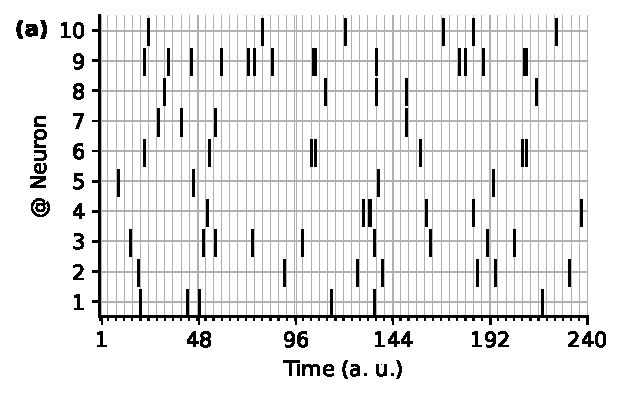
\includegraphics[width=.50\linewidth]{figures/THC_1a_k.pdf}
    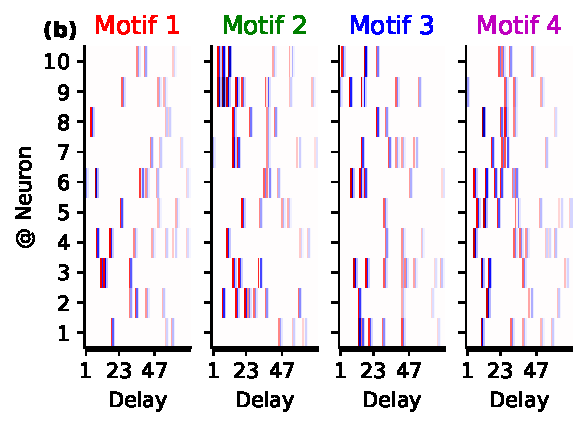
\includegraphics[width=.46\linewidth]{figures/THC_1b.pdf}\\
  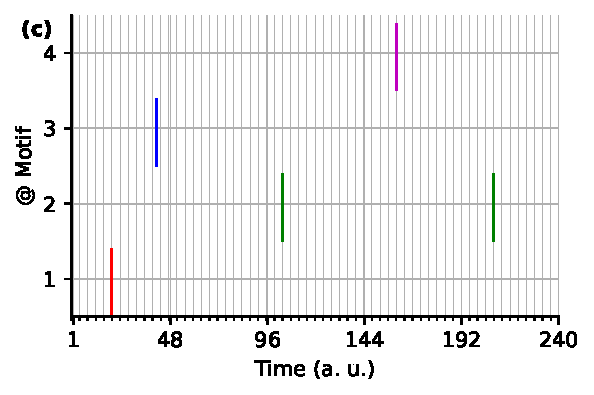
\includegraphics[width=.50\linewidth]{figures/THC_1c.pdf}
    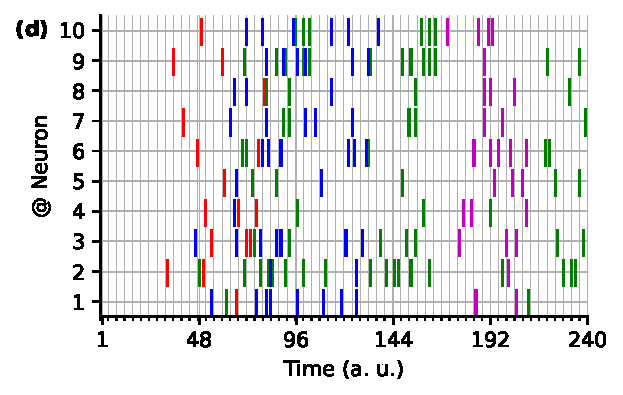
\includegraphics[width=.50\linewidth]{figures/THC_1a.pdf}
  
\caption{\textbf{(a)}~As an illustration for the generative model, we draw a multiunit raster plot synthesized from $4$ different spiking motifs and for $10$ neurons. \textbf{(b)}~We show these motifs, each identified at the top by a different color. Each neuron and $71$ different possible delays is assigned the evidence of activation (red) or deactivation (blue). \textbf{(c)}~The activation in time of the different motifs is then used to define a generative model for drawing a raster plot on the multi-unit address space. \textbf{(d)}~By inverting this model, an inference model can be defined for their efficient detection. The original raster plot can be annotated with each identified spiking motif.
}
\label{fig:THC}
\end{figure}
%---------------------------

% 
Assuming that we know the spiking motifs (as defined by the kernel $\kernel$), the generative model defined above allows to determine the optimal (in the Bayesian sense) inference model for inferring sources $\hat{B}$ when observing a raster plot $A$. Indeed, by using this forward model, it is possible to estimate the logit (inverse of a sigmoid) $\hat{B}(b, t)$ for the presence of a spiking motif of address $b$ and at time $t$ by using the transpose convolution operator. Equivalently, this consists in using the emitting field $\synapse_\presynaddr$ of presynaptic neurons in place of the receptive field $\synapse^\postsynaddr$ of postsynaptic neurons. It thus comes that when observing $A$, then one may infer the logit of the probability as the sum of evidences:
\begin{equation*}
  p(t, \postsynaddr) = \sigma\big(\kernel_\postsynaddrspace(b) + \sum_{\presynaddr,  0 \le \synapticdelay \le D} A(\presynaddr, t-\synapticdelay) \cdot \kernel^T_\presynaddr(\postsynaddr, \synapticdelay) \big)  
\end{equation*}
This also takes the form of a temporal convolution. This assumption holds as long as the kernels are uncorrelated, a condition which is met here numerically by choosing a relatively sparse set of synapses (approximately $1\%$ of active synapses). Finally, we compute $\hat{B}$ by selecting the most likely items. 

One may naturally extend this algorithm when the spiking motifs (that is, the weights) are not known, but that we know the timing and identity of the spiking motifs. Indeed, the equation above is differentiable. 
The underlying metric is the binary cross-entropy, as used in the logistic regression model. In particular, if we consider kernels with similar decreasing exponential time profile, one can prove that this detection model is similar to the method of~\cite{berens_fast_2012}. In our specific case, the difference is that the regression is performed in both dendritic and delay space by extending the summation using a temporal convolution operator. 

%\subsection{Implementation using spiking neurons with heterogeneous delays}
%
% The activation function of our spiking neural is a softmax function implementing a form of  Multinomial Logistic Regression (MLR)~\cite{grimaldi_robust_2022}, in analogy to a spiking Winner-Take-All network~\cite{nessler_bayesian_2013}. 
%It transforms this list of weights into a probability with the following formula:
%$
%Pr(k=\postsynaddr \; \vert \; \timev) =
%\frac 1 Z
%{\exp  (\mathcal{C}^\postsynaddr(\timev) +\bias^\postsynaddr) }
%$ 
%where $\mathcal{C}^\postsynaddr(\timev) = \sum
%\activeweights^\postsynaddr(t)
%$ is the sum of the synaptic weights and $\bias^\postsynaddr$ is the bias linked to neuron $\postsynaddr$. 
%In particular, we expect that some specific motifs may become tightly synchronized as they reach the basal dendritic tree, leading to a high postsynaptic activity which makes it progressively more likely to generate an output spike.
%%
%
% \note{say that it is effortless in biology but difficult on conventional computers}
% In our MLR model with $\Nclass=\Nspeed$ classes, a probability value is predicted for each event at address $\presynaddr_\arank$ and at time $\timev_\arank$ as a softmax function of the linear combination of the list of events on the basal dendrite of a neuron $\postsynaddr$ in association to a specific class. The linear combination can be defined by a set of synapses $\synapse^\postsynaddr$ as described in the heterogeneous delays model. 
%
\section{Results}
%
To quantify the efficiency of this operation, we generated $M=144$ synthetic spiking motifs as random independent kernels over $128$ presynaptic inputs and $D=71$ possible delays. We drew random independent instances of $B$ with a length of $T=1000$ time steps and with on average $1.0$ spike per neuron in each draw. This allowed us to generate raster plots which we use to infer $\hat{B}$. We compute the accuracy as the rate of true positive detections (both for inferring the address and its exact timing) and observe on average $\approx 98\%$ correct detections. We further extended this result by showing how the accuracy would evolve as a function of the number of simultaneous spiking motifs, while keeping the same frequency of occurrence. We show in \fig{model_results}~(Left) that the accuracy of finding the right spiking motif is still above $80\%$ accuracy with more than $1364$ overlapping spiking motifs. Moreover, we show in \fig{model_results}~(Right) that (with $M=144$ spiking motifs fixed) the accuracy increases notably as the temporal depth $D$ of the spiking motif kernel increased, demonstrating quantitatively the computational advantage of using heterogeneous delays. These results were obtained while assuming that we know $W$. However, this is in general not the case, for instance when observing the raster plot of a population of neurons. % In the following, we will define a generic visual task and determine a learning algorithm to solve that challenging task. %Inspired by the k-means algorithm, it is possible to devise a self-supervised learning algorithm. Our preliminary results show that it is possible to retrieve spiking motifs embedded in the data, yet that further analysis is necessary to improve the convergence of the algorithm. In particular, it seems promising to use a sparseness constraint in the inference mechanism such as to remove spurious correlations in the inference.

%---------------------------
\begin{figure}%[t!]
  \centering
  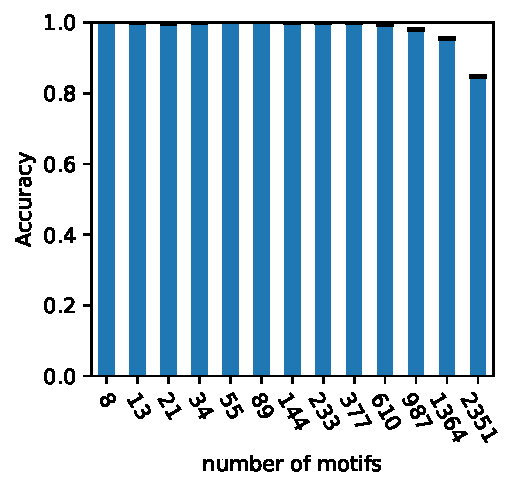
\includegraphics[width=0.480\linewidth]{figures/THC_N_PGs.pdf}
%  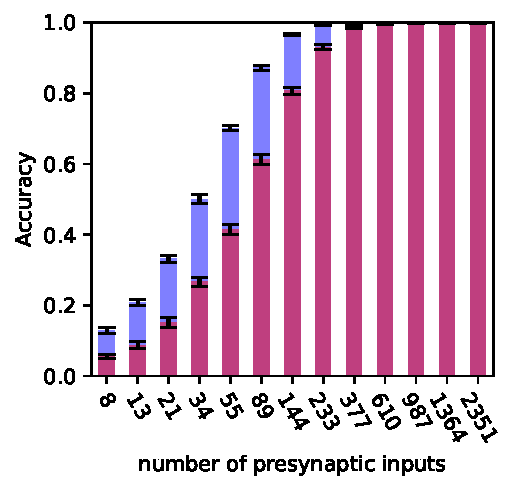
\includegraphics[width=0.320\linewidth]{figures/THC_N_pre.pdf}
  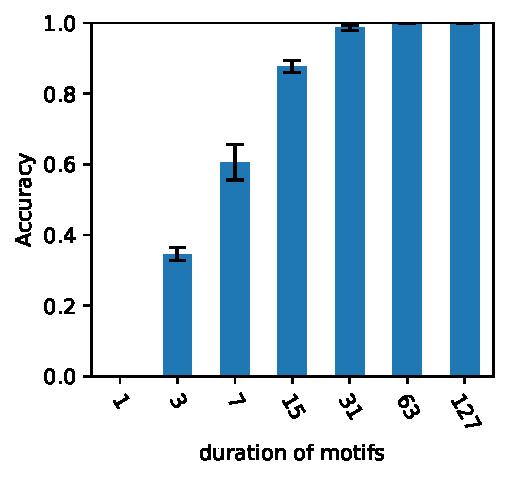
\includegraphics[width=0.480\linewidth]{figures/THC_N_PG_time.pdf}
    \caption{Detecting event-based motifs using spiking neurons with heterogeneous delays. 
Accuracy of detection as a function of  {\bf (Left)}~the number $M$ of kernels, 
    %{\bf (Middle)}~the number of presynaptic neurons, 
    {\bf (Right)}~the temporal depth $D$ of kernels among $M=144$ kernels.
    }
  \label{fig:model_results}
\end{figure}
%---------------------------
%This generative model allows to derive an inference model for the estimation of sources $B$ when observing a raster plot $A$.  In our specific case, the difference with~\cite{russo_cell_2017,stella_3d-spade_2019} is that the regression is performed in both dendritic and delay space by extending the summation with a temporal convolution operator. Using this forward model, it is possible to estimate the logit (inverse of a sigmoid) $\hat{B}(b, t)$ for the presence of a motif at address $b$ and time $t$ by using the transpose convolution operator. Thus, when observing $A$, one can infer $\hat{B} = A \ast W^T$ and select the most activated elements. In particular, if we consider weights $\kernel_b$ with similar decreasing exponential time profiles, we can prove that this is similar to finding the tuning function of L-NL neurons, as used in the method of~\cite{berens_fast_2012}. Assuming that we know the spiking motifs as defined by the $\kernel_b$ matrices, we quantified the accuracy of detecting the occurrence of spiking motifs as the average number of times that the exact address and time were inferred.  To quantify the efficiency of this operation, we generated $M=55$ synthetic spiking motifs as random independent kernels over $128$ presynaptic inputs and $D=71$ possible delays. We drew random independent instances of $B$ with a length of $T=1000$ time steps and with an average of $2.0$ occurrences each. This allowed us to generate raster plots which we used to infer $\hat{B}$. We compute the accuracy as the rate of true positive detections and observe on average about $98\%$ correct spiking motifs for both address and timing.

%We extended this result by showing how accuracy would evolve as a function of the number of simultaneous spiking motifs, while keeping the frequency of occurrence the same. We show in \fig{model_results} that the accuracy of finding the right motif is still above $80\%$ accuracy with more than $1364$ spiking motifs. Moreover, we show in \fig{model_results}-Right that (with $M=55$ spiking motifs fixed) the accuracy increases sharply as the temporal depth $D$ of the spiking motifs is increased. This quantitatively demonstrates the potential of using codes with spiking motifs. 
%
\section{Discussion}
%
In this paper, we have introduced a generic SNN using heterogeneous delays and shown how it can accurately detect spiking motifs. This shows that we can use the precise timing of spikes to improve Neural Comp. 
%
\subsection{Synthesis and Main Contributions}
%%%-----------------------------------------------------------------
To summarize, in this paper we introduced a heterogeneous delay SNN model that we evaluated for optimal detection of event-driven spatiotemporal motifs. We have shown that, when trained on a dataset of synthetic raster images, the model accurately detects the identity and timing of spiking motifs. Let us highlight some innovations in the contributions presented in this paper. First, the generic heterogeneous model is formalized from first principles for optimal detection of the event-based spatiotemporal motifs, while some methods use a correlation-based heuristic~\cite{ghosh_spatiotemporal_2019,yu_stsc-snn_2022}, which we found to be less efficient. Moreover, compared to HOTS~\cite{lagorce_hots_2017}, the weights are explicable as they directly inform on the logit (inverse sigmoid of the probability) of detecting each spatiotemporal spiking motif. Another novelty is that the model learns the weights and the delays simultaneously, while for example the polychronization model~\cite{izhikevich_polychronization_2006} learns only the weights using STDP, while the delays are randomly drawn and their values are frozen. Also, the model is evaluated on a realistic task, while models like the tempotron are tested on simplified problems~\cite{gutig_tempotron_2006}. 
% A striking example is given for the barn owl auditory system: As it hears the sound of a mouse, this sound will generate a specific spiking response in both ears, and specifically, the precise timing between these signals can be used to determine the position of the prey~\cite{goodman_spike-timing-based_2010}. 
\subsection{Main limits}
%%%-----------------------------------------------------------------
We have identified several limitations of our model, which we will now discuss in detail. First, the entire framework is based on discrete time binning, which is incompatible with the continuous nature of biological time. We have used this binning to efficiently implement the framework on conventional hardware, especially GPUs, and in particular to use three-dimensional convolutions. We have tested the effect of the size of the time bin and shown that it has essentially no effect on the results presented in this paper. This is consistent with the relative robustness of other event-based frameworks such as HOTS~\cite{lagorce_hots_2017}, where accuracy was unaffected when the input spikes were subjected to noisy perturbations up to $1~\ms$~\cite{grimaldi_robust_2022}. This suggests the possibility of analytically including a precision term in the temporal value of the input spikes, a mechanism potentially implemented by the filtering implemented by the synaptic time constant of about $5~\ms$. Furthermore, it is possible to circumvent the need for time discretization by using a purely event-based scheme. Indeed, it is not necessary to compute the voltage traces between two spikes~\cite{hanuschkin_general_2010} and it is thus possible to define a purely event-based framework. Such an architecture could provide promising speed gains for the computations.

Another limitation is that this model is purely feed-forward. Thus, the spikes produced by the postsynaptic neurons are generated solely on the basis of information contained in the classical receptive field. However, it is well known that neurons in the same layer can interact via lateral interactions, for example in V1, and that this can be the basis for computational principles~\cite{chavane_revisiting_2022}. For example, the combination of neighboring orientations may contribute to image categorization~\cite{perrinet_edge_2015}. Furthermore, neural information is modulated by feedback information, e.g. to distinguish a figure from its background~\cite{roelfsema_early_2016}, and it has been shown that feedback may be essential for building realistic models of primary visual areas~\cite{boutin_sparse_2020,boutin_effect_2020}, especially to explain non-linear mechanisms~\cite{boutin_pooling_2022}. It is currently not possible to implement these recurrent connections in our implementation (lateral or feedback), mainly due to our use of convolutions. However, the generic theoretical model is able to incorporate them by inserting new spikes into the list of spikes reaching presynaptic addresses. While this is possible in theory, it must be properly adjusted in practice so that these recurrent connections do not amplify neuronal activity outside of a homeostatic state (through extinction or explosion of activity).  

Such recurrent activity would be essential for the implementation of predictive or anticipatory processes. This is essential in a neural system because it contains multiple different delays that require temporal alignment~\cite{hogendoorn_predictive_2019}. This has already been modeled to explain the flash-lag illusion~\cite{khoei_flash-lag_2017}. As noted above, this could be implemented using generalized coordinates (i.e., variables such as position complemented by velocity, acceleration, jerk, \ldots), and ``neurobiologically, using delay operators just means changing synaptic connection strengths to take different mixtures of generalized sensations and their prediction errors''~\cite{perrinet_active_2014}. Our proposed heterogeneous delay model provides an alternative and elegant implementation solution to this problem.''
%
\subsection{Perspectives}
%%%-----------------------------------------------------------------
% learning
The coding results were obtained under the assumption that we know $W$. However, this is generally not the case, e.g. when looking at the neurobiological raster plot of a population of neurons. One perspective would be to extend the model to a fully self-supervised learning paradigm, i.e. without any labeled data~\cite{barlow_unsupervised_1989}. This type of learning is thought to be prevalent in the central nervous system and, assuming the signal is sparse~\cite{olshausen_emergence_1996}, one could extend these Hebbian sparse learning schemes to spikes~\cite{perrinet_emergence_2004,masquelier_competitive_2009}. We expect that this would be particularly useful for exploring neurobiological data~\cite{mackevicius_unsupervised_2019}. Indeed, there is a large literature showing that brain dynamics often organize into stereotyped sequences such as synfire chains~\cite{ikegaya_synfire_2004}, packets~\cite{luczak_sequential_2007}, or hippocampal sequences~\cite{pastalkova_internally_2008,villette_internally_2015}. These motifs are stereotyped and robust, as they can be activated in the same motif from day to day~\cite{haimerl_internal_2019}. In contrast to conventional methods used to process neurobiological data, such an event-based model would be able to answer key questions regarding the representation of information in neurobiological data. Furthermore, it would open possibilities in the field of machine learning, especially in computer vision, to address current key concerns such as robustness to attacks, scalability, interpretability, or energy consumption.

(for a review, see~\cite{grimaldi_precise_2022})




Inspired by the k-means algorithm, it is possible to develop a self-supervised learning algorithm for the automatic detection of spiking motifs. For this, we can draw a random realization for $W$ and define an auto-encoder scheme that, for each grid $A$, infers the sources $B$ and then resynthesizes the corresponding grid. A natural metric is binary cross-entropy, as used in the logistic regression model. Since the model is differentiable, we can optimize $W$ using gradient descent. We can add a homeostatic regularization on the average firing rate of $B$ to ensure that each motif was \emph{a priori} equally activated~\cite{perrinet_role_2010,perrinet_adaptive_2019}. Our preliminary results show that it is possible to retrieve spiking motifs embedded in synthetic data. However, further analysis is needed to improve the convergence of the algorithm and to apply such algorithms to neurobiological data. In particular, it seems promising to use a sparseness constraint in the inference mechanism to remove spurious correlations in the inference.
%
%\subsubsection{Acknowledgements} LP received support from the french government under the France 2030 investment plan, as part of the Initiative d’Excellence d’Aix-Marseille Université – A*MIDEX number AMX-21-RID-025 ``\href{https://laurentperrinet.github.io/grant/polychronies/}{Polychronies}''.
% \printbibliography 
%\bibliographystyle{splncs04}
%\bibliography{ref}
%\bibliography{references}
{%\tiny
\begin{thebibliography}{10}
\providecommand{\url}[1]{\texttt{#1}}
\providecommand{\urlprefix}{URL }
\providecommand{\doi}[1]{}%https://doi.org/#1}

\bibitem{aronov_non-euclidean_2004}
Aronov, D., Victor, J.D.: Non-{Euclidean} properties of spike train metric
  spaces. Physical Review E  \textbf{69}(6),  061905 (Jun 2004).
 % \doi{10.1103/PhysRevE.69.061905}
  
\bibitem{barlow_unsupervised_1989}
Barlow, H.: Unsupervised {Learning}. Neural Comp  \textbf{1}(3),
  295--311 (Sep 1989). %\doi{10.1162/neco.1989.1.3.295},
  
\bibitem{berens_fast_2012}
Berens, P., Ecker, A.S., Cotton, R.J., Ma, W.J., Bethge, M., Tolias, A.S.: A
  {Fast} and {Simple} {Population} {Code} for {Orientation} in {Primate} {V1}.
  Journal of Neuroscience  \textbf{32}(31),  10618--10626 (Aug 2012).
  %%\doi{10/f365rn}
  
\bibitem{boutin_pooling_2022}
Boutin, V., Franciosini, A., Chavane, F., Perrinet, L.U.: Pooling strategies in
  {V1} can account for the functional and structural diversity across species.
  PLOS Computational Biology  \textbf{18}(7),  e1010270 (2022).
  %\doi{10.1371/journal.pcbi.1010270}
  

\bibitem{boutin_sparse_2020}
Boutin, V., Franciosini, A., Chavane, F.Y., Ruffier, F., Perrinet, L.U.: Sparse
  {Deep} {Predictive} {Coding} captures contour integration capabilities of the
  early visual system. PLoS Computational Biology  (May 2020).
  %\doi{10.1371/journal.pcbi.1008629}
 

\bibitem{boutin_effect_2020}
Boutin, V., Franciosini, A., Ruffier, F., Perrinet, L.U.: Effect of top-down
  connections in {Hierarchical} {Sparse} {Coding}. Neural Comp
  \textbf{32}(11),  2279--2309 (Feb 2020). %\doi{10.1162/neco_a_01325}
  
\bibitem{chavane_revisiting_2022}
Chavane, F., Perrinet, L.U., Rankin, J.: Revisiting horizontal connectivity
  rules in {V1}: from like-to-like towards like-to-all. Brain Structure and
  Function  (Feb 2022). %\doi{10.1007/s00429-022-02455-4}
  
\bibitem{ghosh_spatiotemporal_2019}
Ghosh, R., Gupta, A., Tang, S., Soares, A., Thakor, N.: Spatiotemporal
  {Feature} {Learning} for {Event}-{Based} {Vision}. arXiv:1903.06923 [cs]
  (Mar 2019). %{http://arxiv.org/abs/1903.06923}, 00000 arXiv: 1903.06923

\bibitem{goodman_spike-timing-based_2010}
Goodman, D.F.M., Brette, R.: Spike-timing-based computation in sound
  localization. PLoS Comput Biol  \textbf{6}(11) (Nov 2010).
  %\doi{10.1371/journal.pcbi.1000993}
\bibitem{grimaldi_robust_2022}
Grimaldi, A., Boutin, V., Ieng, S.H., Benosman, R., Perrinet, L.: A robust
  event-driven approach to always-on object recognition  (Jan 2022).
  %\doi{10/gn62xd}
  
\bibitem{grimaldi_precise_2022}
Grimaldi, A., Gruel, A., Besnainou, C., Martinet, J., Perrinet, L.U.: Precise
  {Spiking} {Motifs} in {Neurobiological} and {Neuromorphic} {Dat}. Tech. rep.
  (2022). %\doi{10.20944/preprints202211.0332.v1}
  
\bibitem{grun_unitary_2002-1}
Grün, S., Diesmann, M., Aertsen, A.: Unitary events in multiple single-neuron
  spiking activity: {I}. {Detection} and significance. Neural Comp
  \textbf{14}(1),  43--80 (Jan 2002). %\doi{10.1162/089976602753284455},

\bibitem{grun_unitary_2010}
Grün, S., Diesmann, M., Aertsen, A.: Unitary {Event} {Analysis}. In: Grün,
  S., Rotter, S. (eds.) Analysis of {Parallel} {Spike} {Trains}, pp. 191--220.
  Springer US, Boston, MA (2010). %\doi{10.1007/978-1-4419-5675-0_10},

\bibitem{gutig_tempotron_2006}
Gütig, R., Sompolinsky, H.: The tempotron: a neuron that learns spike
  timing–based decisions. Nature Neuroscience  \textbf{9}(3),  420--428 (Mar
  2006). %\doi{10/ch29r4}. %{http://www.nature.com/articles/nn1643/}, 00716

\bibitem{haimerl_internal_2019}
Haimerl, C., Angulo-Garcia, D., Villette, V., Reichinnek, S., Torcini, A.,
  Cossart, R., Malvache, A.: Internal representation of hippocampal neuronal
  population spans a time-distance continuum. Proceedings of the National
  Academy of Sciences  \textbf{116}(15),  7477--7482 (Apr 2019).
  %\doi{10/ghpbm3}. %{https://www.pnas.org/content/116/15/7477}, 00012 
  
\bibitem{hanuschkin_general_2010}
Hanuschkin, A., Kunkel, S., Helias, M., Morrison, A., Diesmann, M.: A {General}
  and {Efficient} {Method} for {Incorporating} {Precise} {Spike} {Times} in
  {Globally} {Time}-{Driven} {Simulations}. Frontiers in Neuroinformatics
  \textbf{4}, ~113 (Oct 2010). %\doi{10.3389/fninf.2010.00113}

\bibitem{hogendoorn_predictive_2019}
Hogendoorn, H., Burkitt, A.N.: Predictive {Coding} with {Neural} {Transmission}
  {Delays}: {A} {Real}-{Time} {Temporal} {Alignment} {Hypothesis}. eneuro
  \textbf{6}(2),  ENEURO.0412--18.2019 (Mar 2019). %\doi{10/ggcrbj} 
\bibitem{ikegaya_synfire_2004}
Ikegaya, Y., Aaron, G., Cossart, R., Aronov, D., Lampl, I., Ferster, D., Yuste,
  R.: Synfire {Chains} and {Cortical} {Songs}: {Temporal} {Modules} of
  {Cortical} {Activity}. Science  \textbf{304}(5670),  559--564 (Apr 2004).
  %\doi{10/djckcn}. %{http://www.science.org/doi/10.1126/science.1093173}, 
\bibitem{izhikevich_polychronization_2006}
Izhikevich, E.M.: Polychronization: {Computation} with spikes. Neural
  Computation  \textbf{18}(2),  245--282 (Feb 2006).
  %\doi{10.1162/089976606775093882} 

\bibitem{kass_statistical_2005}
Kass, R.E., Ventura, V., Brown, E.N.: Statistical issues in the analysis of
  neuronal data. Journal of neurophysiology  \textbf{94}(1),  8--25 (2005).
  %\doi{10.1152/jn.00648.2004}, publisher: American Physiological Society

\bibitem{khoei_flash-lag_2017}
Khoei, M.A., Masson, G.S., Perrinet, L.U.: The {Flash}-{Lag} {Effect} as a
  {Motion}-{Based} {Predictive} {Shift}. PLOS Computational Biology
  \textbf{13}(1),  e1005068 (Jan 2017). %\doi{10.1371/journal.pcbi.1005068}
  
\bibitem{kreuz_measuring_2007}
Kreuz, T., Haas, J.S., Morelli, A., Abarbanel, H.D.I., Politi, A.: Measuring
  spike train synchrony. Journal of Neuroscience Methods  \textbf{165}(1),
  151--161 (Sep 2007). %\doi{10.1016/j.jneumeth.2007.05.031}

\bibitem{lagorce_hots_2017}
Lagorce, X., Orchard, G., Galluppi, F., Shi, B.E., Benosman, R.B.: {HOTS}: {A}
  {Hierarchy} of {Event}-{Based} {Time}-{Surfaces} for {Pattern} {Recognition}.
  IEEE Transactions on Pattern Analysis and Machine Intelligence
  \textbf{39}(7),  1346--1359 (2017). %\doi{10.1109/TPAMI.2016.2574707},

\bibitem{lazar_time_2004}
Lazar, A.A.: Time encoding with an integrate-and-fire neuron with a refractory
  period. Neurocomputing  \textbf{58-60},  53--58 (Jun 2004).
  %\doi{10.1016/j.neucom.2004.01.022},

\bibitem{levakova_review_2015}
Levakova, M., Tamborrino, M., Ditlevsen, S., Lansky, P.: A review of the
  methods for neuronal response latency estimation. Biosystems  \textbf{136},
  23--34 (Oct 2015). %\doi{10.1016/j.biosystems.2015.04.008},

\bibitem{luczak_sequential_2007}
Luczak, A., Barthó, P., Marguet, S.L., Buzsáki, G., Harris, K.D.: Sequential
  structure of neocortical spontaneous activity in vivo. Proceedings of the
  National Academy of Sciences  \textbf{104}(1),  347--352 (Jan 2007).
  %\doi{10.1073/pnas.0605643104}. %{https://www.pnas.org/content/104/1/347},

\bibitem{mackevicius_unsupervised_2019}
Mackevicius, E.L., Bahle, A.H., Williams, A.H., Gu, S., Denisenko, N.I.,
  Goldman, M.S., Fee, M.S.: Unsupervised discovery of temporal sequences in
  high-dimensional datasets, with applications to neuroscience. eLife
  \textbf{8},  e38471 (Feb 2019). %\doi{10.7554/eLife.38471},

\bibitem{masquelier_competitive_2009}
Masquelier, T., Guyonneau, R., Thorpe, S.J.: Competitive {STDP}-{Based} {Spike}
  {Pattern} {Learning}. Neural Comp  \textbf{21}(5),  1259--1276 (May
  2009). %\doi{10/dds34f},

\bibitem{olshausen_emergence_1996}
Olshausen, B.A., Field, D.J.: Emergence of simple-cell receptive field
  properties by learning a sparse code for natural images. Nature
  \textbf{381}(6583),  607--609 (1996). %\doi{10/dvj4qz}

\bibitem{pachitariu_robustness_2018}
Pachitariu, M., Stringer, C., Harris, K.D.: Robustness of {Spike}
  {Deconvolution} for {Neuronal} {Calcium} {Imaging}. The Journal of
  Neuroscience  \textbf{38}(37),  7976--7985 (2018).
  %\doi{10.1523/jneurosci.3339-17.2018}. %{https://doi.org/gd9mcx}, this CSL

\bibitem{pastalkova_internally_2008}
Pastalkova, E., Itskov, V., Amarasingham, A., Buzsáki, G.: Internally
  {Generated} {Cell} {Assembly} {Sequences} in the {Rat} {Hippocampus}. Science \textbf{321}(5894), % 1322--1327 
  (2008).
  %\doi{10.1126/science.1159775}.

\bibitem{perrinet_emergence_2004}
Perrinet, L.: Emergence of filters from natural scenes in a sparse spike coding
  scheme. Neurocomputing  \textbf{58-60}(C),  821--826 (2004).
  %\doi{10.1016/j.neucom.2004.01.133},

\bibitem{perrinet_role_2010}
Perrinet, L.U.: Role of homeostasis in learning sparse representations. Neural
  computation  \textbf{22}(7),  1812--36 (2010).
  %\doi{10.1162/neco.2010.05-08-795}

\bibitem{perrinet_adaptive_2019}
Perrinet, L.U.: An adaptive homeostatic algorithm for the unsupervised learning
  of visual features. Vision  \textbf{3}(3), ~47 (2019). %\doi{10/ggkdks},

\bibitem{perrinet_active_2014}
Perrinet, L.U., Adams, R.A., Friston, K.J.: Active inference, eye movements and
  oculomotor delays. Biological Cybernetics  \textbf{108}(6),  777--801 (Dec
  2014). %\doi{10/f6skjq}. %{https://doi.org/10.1007/s00422-014-0620-8},

\bibitem{perrinet_edge_2015}
Perrinet, L.U., Bednar, J.A.: Edge co-occurrences can account for rapid
  categorization of natural versus animal images. Scientific reports
  \textbf{5},  11400 (2015). %\doi{10.1038/srep11400},
%   tex.ids= Perrinet2015,
%  Perrinet2015d, PerrinetBednar15 tex.bdsk-url-2:
%  https://doi.org/10.1038/srep11400 tex.date-added: 2020-03-27 10:11:37 +0100
%  tex.date-modified: 2020-03-27 10:11:44 +0100 tex.grants: anr-bala-v1
%  tex.preprint: https://hal-amu.archives-ouvertes.fr/hal-01202447
%  tex.url\_code: https://github.com/laurentperrinet/PerrinetBednar15 publisher:
%  Nature Publishing Group url: http://dx.doi.org/10.1038/srep11400

\bibitem{riehle_spike_1997}
Riehle, A., Grun, S., Diesmann, M., Aertsen, A.: Spike synchronization and rate
  modulation differentially involved in motor cortical function. Science  \textbf{278}(5345),  1950--1953 (1997).
  %\doi{10.1126/science.278.5345.1950}
  
\bibitem{roelfsema_early_2016}
Roelfsema, P.R., de~Lange, F.P.: Early visual cortex as a multiscale cognitive
  blackboard. Annual review of vision science  \textbf{2},  131--151 (2016).
  %\doi{10.1146/annurev-vision-111815-114443}, publisher: Annual Reviews

\bibitem{van_rossum_novel_2001}
van Rossum, M.C.: A novel spike distance. Neural Comp  \textbf{13}(4),
  751--763 (2001). %\doi{10.1162/089976601300014321}

\bibitem{russo_cell_2017}
Russo, E., Durstewitz, D.: Cell assemblies at multiple time scales with
  arbitrary lag constellations. eLife  \textbf{6},  e19428 (Jan 2017).
  %\doi{10/f9kxd8}. %{https://doi.org/10.7554/eLife.19428}, tex.ids=  Russo2017 publisher: eLife Sciences Publications, Ltd

\bibitem{stella_comparing_2022}
Stella, A., Bouss, P., Palm, G., Grün, S.: Comparing {Surrogates} to
  {Evaluate} {Precisely} {Timed} {Higher}-{Order} {Spike} {Correlations}.
  eneuro  \textbf{9}(3),  ENEURO.0505--21.2022 (2022).
  %\doi{10.1523/eneuro.0505-21.2022}. %{https://doi.org/gqjvht}, this CSL  Item was generated by Manubot v0.5.2 from its persistent identifier  (standard\_id). standard\_id: doi:10.1523/eneuro.0505-21.2022

\bibitem{stella_3d-spade_2019}
Stella, A., Quaglio, P., Torre, E., Grün, S.: {Significance}
  evaluation of spatio-temporal patterns of various temporal extents.
  Biosystems  \textbf{185},  104022 (2019).
  %\doi{10.1016/j.biosystems.2019.104022}. %{https://doi.org/gpshj2}, this  CSL Item was generated by Manubot v0.5.2 from its persistent identifier  (standard\_id). standard\_id: doi:10.1016/j.biosystems.2019.104022

\bibitem{victor_nature_1996}
Victor, J.D., Purpura, K.P.: Nature and precision of temporal coding in visual
  cortex: a metric-space analysis. Journal of Neurophysiology  \textbf{76}(2),
  1310--1326 (1996). %\doi{10.1152/jn.1996.76.2.1310},
%  \url{https://www.physiology.org/doi/10.1152/jn.1996.76.2.1310}

\bibitem{villette_internally_2015}
Villette, V., Malvache, A., Tressard, T., Dupuy, N., Cossart, R.: Internally
  {Recurring} {Hippocampal} {Sequences} as a {Population} {Template} of
  {Spatiotemporal} {Information}. Neuron  \textbf{88}(2),  357--366 (Oct 2015).
  %\doi{10/f7whnn},
  
\bibitem{williams_point_2020}
Williams, A.H., Degleris, A., Wang, Y., Linderman, S.W.: Point process models
  for sequence detection in high-dimensional neural spike trains. Tech. rep.
  (Oct 2020). %{http://arxiv.org/abs/2010.04875}, 00003 tex.ids=
%  Williams2020a arXiv: 2010.04875 rights:
%  http://creativecommons.org/licenses/by/4.0/

\bibitem{yu_stsc-snn_2022}
Yu, C., Gu, Z., Li, D., Wang, G., Wang, A., Li, E.: {STSC}-{SNN}:
  {Spatio}-{Temporal} {Synaptic} {Connection} with {Temporal} {Convolution} and
  {Attention} for {Spiking} {Neural} {Networks} (Oct 2022),
%  \url{http://arxiv.org/abs/2210.05241}, arXiv:2210.05241 [cs, q-bio, stat]

\end{thebibliography}
}
\end{document}
 